\documentclass{article}

\usepackage{paper}
\theoremstyle{definition}
\newtheorem{definition}{Definition}[section]

\newcommand{\hgraph}{\mathcal{H}}
\newcommand{\nodes}{\mathcal{N}}
\newcommand{\weights}{\mathcal{W}}
\newcommand{\edges}{\mathcal{E}}
\newcommand{\trans}{\mathcal{T}}
\newcommand{\ind}{\mathcal{I}}

\usepackage{kbordermatrix}
\renewcommand{\kbldelim}{(}% Left delimiter
\renewcommand{\kbrdelim}{)}% Right delimiter

\begin{document}
    \title{Notes on Causal Incompatibility Inequalities}
    \author{TC Fraser}{Perimeter Institute for Theoretical Physics, Waterloo, Ontario, Canada}
    \date{July 28th, 2016}
    \abstract{Just trying to flesh out some definitions and ideas regarding causal compatibility inequalities of the Hardy type.}

    \subsection*{Building a Hypergraph From The Marginal Description Matrix}

    Beginning with the triangle scenario,

    \begin{center}
        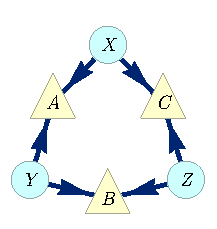
\includegraphics{figures/TriDagRaw.pdf}
    \end{center}

    We inflate to a particular inflation:

    \begin{center}
        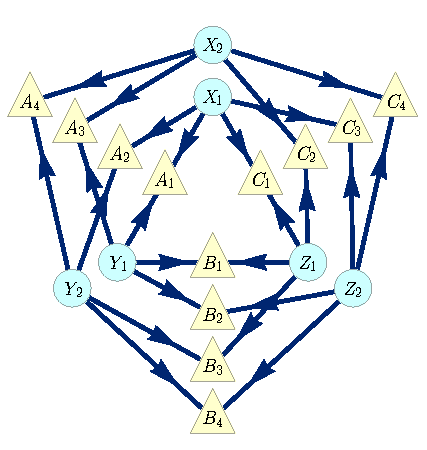
\includegraphics{figures/TriDagFull222.pdf}
    \end{center}

    Then identify the maximal preinjectable sets (with extra notation to denote the factorizations into injectable sets),

    \begin{gather*}
        \bc{\bc{A_1, B_1, C_1}, \bc{A_4, B_4, C_4}} \\
        \bc{\bc{A_1, B_2, C_3}, \bc{A_4, B_3, C_2}} \\
        \bc{\bc{A_2, B_3, C_1}, \bc{A_3, B_2, C_4}} \\
        \bc{\bc{A_2, B_4, C_3}, \bc{A_3, B_1, C_2}} \\
        \bc{\bc{A_1}, \bc{B_3}, \bc{C_4}} \\
        \bc{\bc{A_1}, \bc{B_4}, \bc{C_2}} \\
        \bc{\bc{A_2}, \bc{B_1}, \bc{C_4}} \\
        \bc{\bc{A_2}, \bc{B_2}, \bc{C_2}} \\
        \bc{\bc{A_3}, \bc{B_3}, \bc{C_3}} \\
        \bc{\bc{A_3}, \bc{B_4}, \bc{C_1}} \\
        \bc{\bc{A_4}, \bc{B_1}, \bc{C_3}} \\
        \bc{\bc{A_4}, \bc{B_2}, \bc{C_1}}
    \end{gather*}

    The marginal description matrix $\mathcal{D}$ is a matrix that effectively describes how marginal distributions over the preinjectable sets arise from a joint distribution over all of the observable random variables in the causal model above.

    \begin{definition}{Outcome Spaces}
    Borrowing the notation from Fritz's BBT2, a random variable $v$ has an outcome space denoted $O_v$ corresponding to the set of all possible outcomes of $v$. A particular outcome of $v$ can be denoted as $o\bs{v} \in O_v$. \\

    This notation generalizes to set of random variables $V = \bc{v_1, \ldots, v_{\abs{V}}}$. A \textit{specific} outcome for a set of random variables is denoted
    \[ o\bs{V} = \br{o\bs{v_1}, o\bs{v_2}, \ldots, o\bs{v_{\abs{V}}} } \]
    Whereas the joint outcome space over $V$ is a tensor product of all of the combinations of outcomes,
    \[ O_V = O_{v_1} \otimes \cdots \otimes O_{v_{\abs{V}}} \]
    \end{definition}

    The rows of $\mathcal{D}$ correspond to the elements of the outcome spaces over the preinjectable sets. Let $P_i \in \mathcal{P}$ be a particular preinjectable set of random variables. Take for example,

    \[ P_2 = \bc{A_1, B_2, C_3, A_4, B_3, C_2} \]

    To iterate over the outcome space of $P_2$, we need to define a canonical ordering and the individual outcome spaces. In our case, all observable outcomes have 4 possible outcomes,

    \[ O_{A_1} = O_{A_2} = \cdots = O_{C_4} = \bc{0,1,2,3} \]

    And the canonical ordering is alphanumeric,

    \[ P_2 = \bc{A_1, A_4, B_2, B_3, C_2, C_3} \]

    Therefore for $P_2$ be have $\abs{O_{P_2}} = \prod_{v\in P_2} \abs{O_v} = 4^6 = 4096$ possible outcomes. In total over all the preinjectable sets we have,

    \[ \sum_{i=1}^{12} \abs{O_{P_i}} = 4 \cdot \br{4^6} + 8\cdot\br{4^3} = 16,896 \]

    Rows in the marginal description matrix $\mathcal{D}$. The columns in the marginal description matrix $\mathcal{D}$ correspond to the outcomes over all of the observable variables,

    \[ X = \br{A_1, A_2, A_3, \cdots, C_3, C_4} \]
    \[ \abs{O_X} = 4^{12} = 16,777,216 \]

    The entries of $\mathcal{D}$ are either $1$ or $0$. A $1$ is placed whenever an outcome over the preinjectable set is \textit{extendable} to the corresponding outcome over $X$.

    Explicitly,

    \[ \br{o\bs{A_1} = 2, o\bs{B_3} = 0, o\bs{C_4} = 0} \]

    Is extendable to lots of possible outcomes,

    \[ 4^{\abs{O_{X}} - \abs{O_{P_5}}} = 262144 \]

    \begin{center}
        \begin{tabular}{|c|c|c|c|c|c|c|c|c|c|c|c|}
            \hline
            $A_1$ & $A_2$ & $A_3$ & $A_4$ & $B_1$ & $B_2$ & $B_3$ & $B_4$ & $C_1$ & $C_2$ & $C_3$ & $C_4$ \\
            \hline
            \hline
            - & 2 & - & - & - & - & 0 & - & - & - & - & 0 \\
            $\vdots$ & $\vdots$ & $\vdots$ & $\vdots$ & $\vdots$ & $\vdots$ & $\vdots$ & $\vdots$ & $\vdots$ & $\vdots$ & $\vdots$ & $\vdots$ \\
            0 & 2 & 1 & 2 & 3 & 2 & 0 & 3 & 2 & 1 & 0 & 0 \\
            3 & 2 & 2 & 0 & 3 & 2 & 0 & 1 & 2 & 0 & 0 & 0 \\
            \hline
        \end{tabular}
    \end{center}
    % \[ \br{o\bs{A_1} = 2, o\bs{B_3} = 0, o\bs{C_4} = 0} \]

    \subsection*{Deriving Inequalities}
    In order to identify the contrapositive forms of a logical tautologies over the preinjectable outcomes, we are searching for cases where a particular event $E_0$ implies the occurrence of at least one of the other set of events. This possibilistic constraint,

    \[ E_0 \implies E_1 \lor \cdots \lor E_k = \bigvee_{i=1}^{k} E_i \]

    Translates to a weaker description in terms of a probabilistic constraint,
    \[ P\br{E_0} \leq P\br{\bigvee_{i=1}^{k} E_i} \leq \sum_{i=1}^{k} P\br{E_i}\]

    The events $E_i$ in this case correspond to joint outcomes of a particular preinjectable set.

    \[ E_i \longleftrightarrow o\bs{P_j} \]

    To build logical tautologies for a particular $E_0 = o\bs{P_2}$, one needs to find other events over the rows of $\mathcal{D}$ that cover all of the possible extensions of $E_0$. To explain this further,

    \begin{itemize}
        \item Assume that the random variables $X$ over the inflation DAG admit a joint distribution
        \item If say $E_0 = o\bs{P_5} = \br{o\bs{A_1} = 2, o\bs{B_3} = 0, o\bs{C_4} = 0}$ happened to occur, then it must correspond to the fact that at a particular outcome occurred $o\bs{X}$ that is expendable/compatible with $o\bs{P_5}$ (under specifying the remaining $X \setminus P_5$ random variables)
        \item Given this outcome $o\bs{X}$ occurred, then some other marginal outcomes over other preinjectable sets had to occur $o\bs{P_i}, i \neq 5$
        \item If you can find a set $\bc{E_i}$ of these \textit{possibly implied} outcomes over the preinjectable sets that covers all of the ways to extend $E_0$, then at least one of the elements of $\bc{E_i}$ \textit{had to have occured}.
    \end{itemize}

    Finding a set of outcomes over the preinjectable sets that accomplishes this gives us a compatibility inequality $I'$ over the inflation random variables $X$. \\

    If $I'$ is satisfied, then compatibility between $X$ and the inflation DAG is not ruled out. If $I'$ is violated, then an assumption made above must be wrong. Namely, that there exists a joint distribution over $X$. \\

    Furthermore, since $I'$ is written in terms of distributions over the preinjectable sets, this translates directly to an analogous incompatibility inequality $I$ over the deflated random variables and the deflated DAG. \\

    \subsection*{Techniques}


    \begin{definition}{Hypergraph:}
        A \textit{Hypergraph} $\hgraph$ is an ordered tuple $\br{\nodes, \edges}$ of \textit{nodes} and \textit{edges} respectively where the nodes can represent any object and the edges are subsets of nodes.

        For convenience of notation, one defines an index set over the nodes and edges of a hypergraph $\hgraph$ denoted $\ind_\nodes$ and $\ind_\edges$ respectively.

        \[ \nodes = \bc{n_i \mid i \in \ind_\nodes} \]
        \[ \edges = \bc{e_i \mid i \in \ind_\edges, e_i \subseteq \nodes} \]

        \textit{Note:} Where the index for an edge or node is arbitrary, it will be omitted. \\

        There is a dual correspondence between edges $e \in \edges$ and nodes $n \in \nodes$ in a Hypergraph. An edge $e$ is viewed as a set of nodes $\bc{n_i}$, and a node $n$ can be viewed as the set of edges $\bc{e_i}$ that contain it.
    \end{definition}

    \begin{definition}{Hypergraph Transversal:}
        A \textit{Transversal} $\trans$ of a Hypergraph $\hgraph$ is a set of nodes $\trans \subseteq \nodes$ that intersect with every edge in $\edges$.
        \[ \trans = \bc{n_i \in \nodes \mid i \in \ind_\trans } \quad \forall e \in \edges : \trans \cap e \neq \emptyset \]
    \end{definition}

    \begin{definition}{Weighted Hypergraph:}
        A \textit{Weighted Hypergraph} $\hgraph_\weights$ is a regular hypergraph equipped with a set of weights $\weights$ ascribed to each node such that a weighted hypergraph is written as a triplet $\br{\weights, \nodes, \edges}$.
        \[ \weights = \bc{w_i \mid i \in \ind_\nodes, w_i \in \R} \]
        One would say that a particular node $n_i$ carries weight $w_i$.
    \end{definition}

    \begin{definition}{Weighted Transversal:}
        A \textit{weighted transversal} of a weighted hypergraph $\hgraph_\weights$ is a transversal $\trans$ of the unweighted hypergraph $\hgraph$ and a real number $t$ (denoted $\trans_t$) such that the sum of the node weights of the transversal is bounded by $t$.

        \[ \trans_t = \bcm{n_i}{i \in \ind_\trans, \sum_{j\in\ind_\trans} w_j \leq t} \]
    \end{definition}

    \subsection*{Sparse Matrix As A Hypergraph Data Structure}

    To illustrate how a general hypergraph can be viewed as a matrix, consider the hypergraph,

    \begin{gather*}
       \hgraph = \br{\nodes, \edges} \\
       \nodes = \bc{n_1, n_2, n_3, n_4, n_5} \\
       \edges = \bc{e_1 = \bc{n_1, n_3}, e_2 = \bc{n_2}, e_3 = \bc{n_5}, e_4 = \bc{n_2, n_4, n_5}, e_5 = \bc{n_1, n_2}, e_6 = \bc{n_1, n_4}}
    \end{gather*}

    That can be casted as a matrix:

    \[ M_\hgraph = \kbordermatrix{
        & e_1 & e_2 & e_3 & e_4 & e_5 & e_6 \\
        n_1 & 1 & 0 & 0 & 0 & 1 & 1 \\
        n_2 & 0 & 1 & 0 & 1 & 1 & 0 \\
        n_3 & 1 & 0 & 0 & 0 & 0 & 0 \\
        n_4 & 0 & 0 & 0 & 1 & 0 & 1 \\
        n_5 & 0 & 0 & 1 & 1 & 0 & 0
    } \]

    The Dual-dual relation as a matrix.
    \[ \br{\hgraph^*}^* \Leftrightarrow \br{M_\hgraph^T}^T \]

    \section*{Reducing The Size of The Hypergraph}

    Beginning with the marginal description matrix $\mathcal{D}$, one obtains a hypergraph $\hgraph$ to transverse for a particular antecedent $E_0 = o\bs{P_i}$ by building a partial hypergraph out of the extendable outcomes (edges) of $O_X$
    and the then a sub-hypergraph over the contractable outcomes (nodes) of $O_{P}$.

    \[ \cdots \]

    \textbf{Reduced Hypergraph}
    \begin{center}
        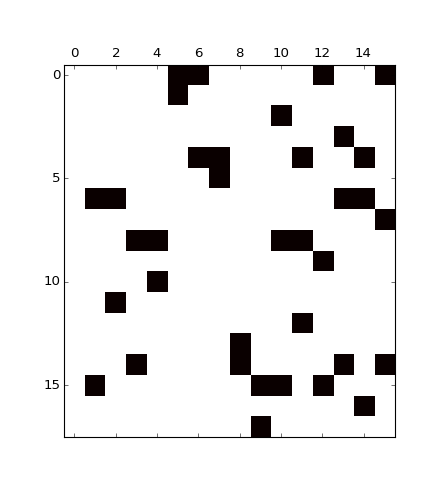
\includegraphics[width=3in]{figures/reduced_hgraph.png}
    \end{center}

    \subsubsection*{Examples}

    As an example of a derived inequality,

    \[ P_{ABC}\br{002}P_{ABC}\br{003} \leq P_{A}(0)P_{B}(0)P_{C}(3) + P_{A}(0)P_{B}(1)P_{C}(3) + P_{A}(0)P_{B}(2)P_{C}(3) + P_{A}(0)P_{B}(3)P_{C}(3) \]

    Ends up being fundamentally trivial. $O_B$ is covered on the RHS,

    \[ P_{ABC}\br{002}P_{ABC}\br{003} \leq P_{A}(0)P_{C}(3) \]

    Now notice that marginalization never decreases probabilistic values,
    \[P_{ABC}\br{002} \leq P_{A}(0) \qquad P_{ABC}\br{003} \leq P_{C}(3) \]

    However, we have derived numerous ($\approx 100,000$) inequalities. Using this technique, we can just keep running the algorithm and find many, many, many more.

    \subsubsection*{Example of A Non-Trivial Inequality}

    \[ P_{ABC} = \f{1}{12}\br{\bs{012} + \bs{201} + \bs{120} + \bs{123} + \bs{312} + \bs{231} + \bs{230} + \bs{023} + \bs{302} + \bs{301} + \bs{130} + \bs{013}} \]

    \[ P(012)P(130) \leq \]
    % P(A_0B_1C_2)P(A_1B_3C_0) \\leq
    \begin{gather*}
    2P(000)P(102) + 2P(000)P(112) + 2P(000)P(122) + 2P(000)P(132) + \\
    2P(010)P(102) + 2P(010)P(112) + 2P(010)P(122) + 2P(010)P(132) + \\
    2P(020)P(102) + 2P(020)P(122) + 2P(020)P(132) + 2P(022)P(110) + \\
    2P(032)P(100) + 2P(032)P(110) + 2P(032)P(120) + P(000)P(002) + \\
    P(000)P(012) + P(000)P(022) + P(000)P(032) + P(000)P(101) + \\
    P(000)P(103) + P(000)P(111) + P(000)P(113) + P(000)P(121) + \\
    P(000)P(123) + P(000)P(131) + P(000)P(133) + P(001)P(100) + \\
    P(001)P(101) + P(001)P(102) + P(001)P(103) + P(001)P(110) + \\
    P(001)P(111) + P(001)P(112) + P(001)P(113) + P(001)P(120) + \\
    P(001)P(121) + P(001)P(122) + P(001)P(123) + P(001)P(130) + \\
    P(001)P(131) + P(001)P(132) + P(001)P(133) + P(002)P(010) + \\
    P(002)P(020) + P(002)P(100) + P(002)P(101) + P(002)P(102) + \\
    P(002)P(110) + P(002)P(111) + P(002)P(112) + P(002)P(120) + \\
    P(002)P(121) + P(002)P(122) + P(002)P(131) + P(002)P(132) + \\
    P(002)P(200) + P(002)P(210) + P(002)P(220) + P(002)P(300) + \\
    P(002)P(310) + P(002)P(320) + P(003)P(101) + P(003)P(102) + \\
    P(003)P(111) + P(003)P(112) + P(003)P(121) + P(003)P(122) + \\
    P(003)P(131) + P(003)P(132) + P(010)P(012) + P(010)P(022) + \\
    P(010)P(032) + P(010)P(101) + P(010)P(103) + P(010)P(111) + \\
    P(010)P(113) + P(010)P(121) + P(010)P(123) + P(010)P(131) + \\
    P(010)P(133) + P(010)P(230) + P(010)P(232) + P(010)P(233) + \\
    P(010)P(330) + P(010)P(332) + P(010)P(333) + P(011)P(100) + \\
    P(011)P(101) + P(011)P(102) + P(011)P(103) + P(011)P(110) + \\
    P(011)P(111) + P(011)P(112) + P(011)P(113) + P(011)P(120) + \\
    P(011)P(121) + P(011)P(122) + P(011)P(123) + P(011)P(130) + \\
    P(011)P(131) + P(011)P(132) + P(011)P(133) + P(012)P(100) + \\
    P(012)P(101) + P(012)P(102) + P(012)P(110) + P(012)P(111) + \\
    P(012)P(112) + P(012)P(121) + P(012)P(122) + P(012)P(131) + \\
    P(012)P(132) + P(012)P(200) + P(012)P(210) + P(012)P(300) + \\
    P(012)P(310) + P(013)P(101) + P(013)P(102) + P(013)P(111) + \\
    P(013)P(112) + P(013)P(121) + P(013)P(122) + P(013)P(131) + \\
    P(013)P(132) + P(013)P(232) + P(013)P(233) + P(013)P(332) + \\
    P(013)P(333) + P(020)P(022) + P(020)P(032) + P(020)P(101) + \\
    P(020)P(103) + P(020)P(110) + P(020)P(111) + P(020)P(112) + \\
    P(020)P(113) + P(020)P(121) + P(020)P(123) + P(020)P(131) + \\
    P(020)P(133) + P(021)P(100) + P(021)P(101) + P(021)P(102) + \\
    P(021)P(103) + P(021)P(110) + P(021)P(111) + P(021)P(112) + \\
    P(021)P(113) + P(021)P(120) + P(021)P(121) + P(021)P(122) + \\
    P(021)P(123) + P(021)P(130) + P(021)P(131) + P(021)P(132) + \\
    P(021)P(133) + P(022)P(100) + P(022)P(101) + P(022)P(102) + \\
    P(022)P(111) + P(022)P(112) + P(022)P(113) + P(022)P(120) + \\
    P(022)P(121) + P(022)P(122) + P(022)P(131) + P(022)P(132) + \\
    P(022)P(200) + P(022)P(210) + P(022)P(220) + P(022)P(300) + \\
    P(022)P(310) + P(022)P(320) + P(023)P(101) + P(023)P(102) + \\
    P(023)P(110) + P(023)P(111) + P(023)P(112) + P(023)P(113) + \\
    P(023)P(121) + P(023)P(122) + P(023)P(131) + P(023)P(132) + \\
    P(030)P(100) + P(030)P(101) + P(030)P(102) + P(030)P(103) + \\
    P(030)P(110) + P(030)P(111) + P(030)P(112) + P(030)P(113) + \\
    P(030)P(120) + P(030)P(121) + P(030)P(122) + P(030)P(123) + \\
    P(030)P(130) + P(030)P(131) + P(030)P(132) + P(030)P(133) + \\
    P(031)P(100) + P(031)P(101) + P(031)P(102) + P(031)P(103) + \\
    P(031)P(110) + P(031)P(111) + P(031)P(112) + P(031)P(113) + \\
    P(031)P(120) + P(031)P(121) + P(031)P(122) + P(031)P(123) + \\
    P(031)P(130) + P(031)P(131) + P(031)P(132) + P(031)P(133) + \\
    P(032)P(101) + P(032)P(102) + P(032)P(103) + P(032)P(111) + \\
    P(032)P(112) + P(032)P(113) + P(032)P(121) + P(032)P(122) + \\
    P(032)P(123) + P(032)P(130) + P(032)P(131) + P(032)P(132) + \\
    P(032)P(133) + P(032)P(200) + P(032)P(210) + P(032)P(220) + \\
    P(032)P(300) + P(032)P(310) + P(032)P(320) + P(033)P(100) + \\
    P(033)P(101) + P(033)P(102) + P(033)P(103) + P(033)P(110) + \\
    P(033)P(111) + P(033)P(112) + P(033)P(113) + P(033)P(120) + \\
    P(033)P(121) + P(033)P(122) + P(033)P(123) + P(033)P(130) + \\
    P(033)P(131) + P(033)P(132) + P(033)P(133) + P(100)P(102) + \\
    P(100)P(112) + P(100)P(122) + P(100)P(132) + P(102)P(110) + \\
    P(102)P(120) + P(102)P(200) + P(102)P(210) + P(102)P(220) + \\
    P(102)P(300) + P(102)P(310) + P(102)P(320) + P(110)P(112) + \\
    P(110)P(122) + P(110)P(132) + P(110)P(230) + P(110)P(232) + \\
    P(110)P(233) + P(110)P(330) + P(110)P(332) + P(110)P(333) + \\
    P(112)P(200) + P(112)P(210) + P(112)P(300) + P(112)P(310) + \\
    P(113)P(232) + P(113)P(233) + P(113)P(332) + P(113)P(333) + \\
    P(120)P(122) + P(120)P(132) + P(122)P(200) + P(122)P(210) + \\
    P(122)P(220) + P(122)P(300) + P(122)P(310) + P(122)P(320) + \\
    P(132)P(200) + P(132)P(210) + P(132)P(220) + P(132)P(300) + \\
    P(132)P(310) + P(132)P(320) + P(210)P(230) + P(210)P(232) + \\
    P(210)P(233) + P(210)P(330) + P(210)P(332) + P(210)P(333) + \\
    P(213)P(232) + P(213)P(233) + P(213)P(332) + P(213)P(333) + \\
    P(230)P(310) + P(232)P(310) + P(232)P(313) + P(233)P(310) + \\
    P(233)P(313) + P(310)P(330) + P(310)P(332) + P(310)P(333) + \\
    P(313)P(332) + P(313)P(333)
    \end{gather*}

    \subsubsection*{Example of A Fritz Inequality}
    \[ P \defined P_{ABC} \]
    \[ P(000)P(233) \leq \ldots \]
        %
    \begin{gather*}
    2P(001)P(230) + 2P(001)P(232) + 2P(003)P(230) + 2P(003)P(232) + \\
    2P(020)P(203) + 2P(020)P(213) + 2P(020)P(233) + 2P(030)P(203) + \\
    2P(030)P(213) + 2P(030)P(223) + 2P(030)P(233) + P(000)P(003) + \\
    P(000)P(013) + P(000)P(023) + P(000)P(033) + P(000)P(103) + \\
    P(000)P(113) + P(000)P(123) + P(000)P(133) + P(000)P(202) + \\
    P(000)P(203) + P(000)P(212) + P(000)P(213) + P(000)P(222) + \\
    P(000)P(230) + P(000)P(232) + P(000)P(303) + P(000)P(313) + \\
    P(000)P(330) + P(001)P(200) + P(001)P(201) + P(001)P(202) + \\
    P(001)P(203) + P(001)P(210) + P(001)P(211) + P(001)P(212) + \\
    P(001)P(213) + P(001)P(220) + P(001)P(221) + P(001)P(222) + \\
    P(001)P(223) + P(001)P(231) + P(001)P(233) + P(001)P(330) + \\
    P(001)P(332) + P(002)P(200) + P(002)P(202) + P(002)P(210) + \\
    P(002)P(212) + P(002)P(220) + P(002)P(222) + P(002)P(230) + \\
    P(002)P(232) + P(003)P(010) + P(003)P(020) + P(003)P(030) + \\
    P(003)P(100) + P(003)P(110) + P(003)P(120) + P(003)P(130) + \\
    P(003)P(200) + P(003)P(201) + P(003)P(202) + P(003)P(203) + \\
    P(003)P(210) + P(003)P(211) + P(003)P(212) + P(003)P(213) + \\
    P(003)P(220) + P(003)P(221) + P(003)P(222) + P(003)P(223) + \\
    P(003)P(231) + P(003)P(233) + P(003)P(330) + P(003)P(332) + \\
    P(010)P(013) + P(010)P(023) + P(010)P(103) + P(010)P(113) + \\
    P(010)P(123) + P(010)P(202) + P(010)P(203) + P(010)P(212) + \\
    P(010)P(213) + P(010)P(222) + P(010)P(232) + P(010)P(303) + \\
    P(010)P(313) + P(011)P(200) + P(011)P(201) + P(011)P(202) + \\
    P(011)P(203) + P(011)P(210) + P(011)P(211) + P(011)P(212) + \\
    P(011)P(213) + P(011)P(220) + P(011)P(221) + P(011)P(222) + \\
    P(011)P(223) + P(011)P(230) + P(011)P(231) + P(011)P(232) + \\
    P(011)P(233) + P(012)P(200) + P(012)P(202) + P(012)P(210) + \\
    P(012)P(212) + P(012)P(220) + P(012)P(222) + P(012)P(230) + \\
    P(012)P(232) + P(013)P(020) + P(013)P(030) + P(013)P(100) + \\
    P(013)P(110) + P(013)P(120) + P(013)P(130) + P(013)P(200) + \\
    P(013)P(201) + P(013)P(202) + P(013)P(203) + P(013)P(210) + \\
    P(013)P(211) + P(013)P(212) + P(013)P(213) + P(013)P(220) + \\
    P(013)P(221) + P(013)P(222) + P(013)P(223) + P(013)P(230) + \\
    P(013)P(231) + P(013)P(232) + P(013)P(233) + P(020)P(023) + \\
    P(020)P(033) + P(020)P(103) + P(020)P(113) + P(020)P(123) + \\
    P(020)P(133) + P(020)P(200) + P(020)P(201) + P(020)P(202) + \\
    P(020)P(210) + P(020)P(211) + P(020)P(212) + P(020)P(222) + \\
    P(020)P(223) + P(020)P(230) + P(020)P(231) + P(020)P(232) + \\
    P(020)P(303) + P(020)P(313) + P(020)P(323) + P(020)P(333) + \\
    P(021)P(200) + P(021)P(201) + P(021)P(202) + P(021)P(203) + \\
    P(021)P(210) + P(021)P(211) + P(021)P(212) + P(021)P(213) + \\
    P(021)P(220) + P(021)P(221) + P(021)P(222) + P(021)P(223) + \\
    P(021)P(230) + P(021)P(231) + P(021)P(232) + P(021)P(233) + \\
    P(022)P(200) + P(022)P(202) + P(022)P(203) + P(022)P(210) + \\
    P(022)P(212) + P(022)P(213) + P(022)P(220) + P(022)P(222) + \\
    P(022)P(230) + P(022)P(232) + P(023)P(030) + P(023)P(100) + \\
    P(023)P(110) + P(023)P(120) + P(023)P(130) + P(023)P(200) + \\
    P(023)P(201) + P(023)P(202) + P(023)P(203) + P(023)P(210) + \\
    P(023)P(211) + P(023)P(212) + P(023)P(213) + P(023)P(220) + \\
    P(023)P(221) + P(023)P(222) + P(023)P(223) + P(023)P(230) + \\
    P(023)P(231) + P(023)P(232) + P(023)P(233) + P(030)P(033) + \\
    P(030)P(103) + P(030)P(113) + P(030)P(123) + P(030)P(133) + \\
    P(030)P(200) + P(030)P(201) + P(030)P(202) + P(030)P(210) + \\
    P(030)P(211) + P(030)P(212) + P(030)P(220) + P(030)P(221) + \\
    P(030)P(222) + P(030)P(230) + P(030)P(231) + P(030)P(232) + \\
    P(030)P(303) + P(030)P(313) + P(030)P(323) + P(030)P(333) + \\
    P(031)P(200) + P(031)P(201) + P(031)P(202) + P(031)P(203) + \\
    P(031)P(210) + P(031)P(211) + P(031)P(212) + P(031)P(213) + \\
    P(031)P(220) + P(031)P(221) + P(031)P(222) + P(031)P(223) + \\
    P(031)P(230) + P(031)P(231) + P(031)P(232) + P(031)P(233) + \\
    P(032)P(200) + P(032)P(201) + P(032)P(202) + P(032)P(203) + \\
    P(032)P(210) + P(032)P(211) + P(032)P(212) + P(032)P(213) + \\
    P(032)P(220) + P(032)P(222) + P(032)P(230) + P(032)P(232) + \\
    P(032)P(301) + P(033)P(100) + P(033)P(120) + P(033)P(130) + \\
    P(033)P(200) + P(033)P(201) + P(033)P(202) + P(033)P(203) + \\
    P(033)P(210) + P(033)P(211) + P(033)P(212) + P(033)P(213) + \\
    P(033)P(220) + P(033)P(221) + P(033)P(222) + P(033)P(223) + \\
    P(033)P(230) + P(033)P(231) + P(033)P(232) + P(033)P(233) + \\
    P(100)P(103) + P(100)P(113) + P(100)P(123) + P(100)P(133) + \\
    P(100)P(203) + P(100)P(213) + P(100)P(223) + P(100)P(230) + \\
    P(100)P(233) + P(100)P(303) + P(100)P(313) + P(100)P(330) + \\
    P(101)P(230) + P(101)P(232) + P(101)P(330) + P(101)P(332) + \\
    P(103)P(110) + P(103)P(120) + P(103)P(130) + P(103)P(230) + \\
    P(103)P(232) + P(103)P(330) + P(103)P(332) + P(110)P(113) + \\
    P(110)P(123) + P(110)P(203) + P(110)P(213) + P(110)P(223) + \\
    P(110)P(303) + P(110)P(313) + P(113)P(120) + P(113)P(130) + \\
    P(120)P(123) + P(120)P(133) + P(120)P(203) + P(120)P(213) + \\
    P(120)P(223) + P(120)P(233) + P(120)P(303) + P(120)P(313) + \\
    P(120)P(323) + P(123)P(130) + P(130)P(133) + P(130)P(203) + \\
    P(130)P(213) + P(130)P(223) + P(130)P(233) + P(130)P(303) + \\
    P(130)P(313) + P(132)P(301) + P(132)P(303) + P(200)P(230) + \\
    P(200)P(330) + P(201)P(230) + P(201)P(232) + P(201)P(330) + \\
    P(201)P(332) + P(203)P(230) + P(203)P(232) + P(203)P(330) + \\
    P(203)P(332) + P(230)P(300) + P(230)P(301) + P(230)P(303) + \\
    P(232)P(301) + P(232)P(303) + P(300)P(330) + P(301)P(330) + \\
    P(301)P(332) + P(303)P(330) + P(303)P(332)
    \end{gather*}

    \section*{Symmetric Inequality}

    \[ 2P(000)P(233) + 2P(000)P(323) + 2P(000)P(332) \leq \]

    \begin{gather*}
        2P(000)P(003) + 2P(000)P(022) + 2P(000)P(030) + 2P(000)P(033) + 2P(000)P(113) +\\
        2P(000)P(122) + 2P(000)P(131) + 2P(000)P(133) + 2P(000)P(202) + 2P(000)P(212) +\\
        2P(000)P(220) + 2P(000)P(221) + 2P(000)P(223) + 2P(000)P(232) + 2P(000)P(300) +\\
        2P(000)P(303) + 2P(000)P(311) + 2P(000)P(313) + 2P(000)P(322) + 2P(000)P(330) +\\
        2P(000)P(331) + 2P(001)P(220) + 2P(001)P(221) + 2P(001)P(222) + 2P(001)P(223) +\\
        2P(001)P(330) + 2P(001)P(331) + 2P(001)P(332) + 2P(002)P(020) + 2P(002)P(110) +\\
        2P(002)P(200) + 2P(002)P(220) + 2P(002)P(221) + 2P(002)P(222) + 2P(002)P(223) +\\
        2P(002)P(330) + 2P(002)P(331) + 2P(002)P(332) + 2P(002)P(333) + 2P(003)P(030) +\\
        2P(003)P(110) + 2P(003)P(220) + 2P(003)P(221) + 2P(003)P(222) + 2P(003)P(223) +\\
        2P(003)P(300) + 2P(003)P(330) + 2P(003)P(331) + 2P(003)P(332) + 2P(003)P(333) +\\
        2P(010)P(202) + 2P(010)P(212) + 2P(010)P(222) + 2P(010)P(232) + 2P(010)P(303) +\\
        2P(010)P(313) + 2P(010)P(323) + 2P(011)P(200) + 2P(011)P(211) + 2P(011)P(222) +\\
        2P(011)P(233) + 2P(011)P(300) + 2P(011)P(311) + 2P(011)P(322) + 2P(012)P(210) +\\
        2P(013)P(310) + 2P(020)P(101) + 2P(020)P(200) + 2P(020)P(202) + 2P(020)P(212) +\\
        2P(020)P(222) + 2P(020)P(232) + 2P(020)P(303) + 2P(020)P(313) + 2P(020)P(323) +\\
        2P(020)P(333) + 2P(021)P(201) + 2P(022)P(100) + 2P(022)P(200) + 2P(022)P(202) +\\
        2P(022)P(220) + 2P(022)P(222) + 2P(022)P(300) + 2P(023)P(203) + 2P(023)P(320) +\\
        2P(030)P(101) + 2P(030)P(202) + 2P(030)P(212) + 2P(030)P(222) + 2P(030)P(232) +\\
        2P(030)P(300) + 2P(030)P(303) + 2P(030)P(313) + 2P(030)P(323) + 2P(030)P(333) +\\
        2P(031)P(301) + 2P(032)P(230) + 2P(032)P(302) + 2P(033)P(100) + 2P(033)P(200) +\\
        2P(033)P(211) + 2P(033)P(222) + 2P(033)P(233) + 2P(033)P(300) + 2P(033)P(303) +\\
        2P(033)P(322) + 2P(033)P(330) + 2P(100)P(122) + 2P(100)P(133) + 2P(100)P(222) +\\
        2P(100)P(233) + 2P(100)P(322) + 2P(101)P(121) + 2P(101)P(131) + 2P(101)P(222) +\\
        2P(101)P(232) + 2P(101)P(323) + 2P(102)P(120) + 2P(103)P(130) + 2P(110)P(112) +\\
        2P(110)P(113) + 2P(110)P(222) + 2P(110)P(223) + 2P(110)P(332) + 2P(112)P(330) +\\
        2P(121)P(303) + 2P(122)P(200) + 2P(122)P(300) + 2P(133)P(200) + 2P(133)P(300) +\\
        2P(200)P(222) + 2P(200)P(233) + 2P(200)P(322) + 2P(200)P(333) + 2P(202)P(220) +\\
        2P(202)P(222) + 2P(203)P(230) + 2P(220)P(222) + 2P(222)P(300) + 2P(222)P(303) +\\
        2P(222)P(330) + 2P(223)P(330) + 2P(232)P(303) + 2P(233)P(300) + 2P(300)P(322) +\\
        2P(300)P(333) + 2P(302)P(320) + 2P(303)P(323) + 2P(303)P(330) + 2P(330)P(332) +\\
        6P(000)P(222) + P(000)P(013) + P(000)P(023) + P(000)P(031) + P(000)P(032) +\\
        P(000)P(103) + P(000)P(123) + P(000)P(130) + P(000)P(132) + P(000)P(203) +\\
        P(000)P(213) + P(000)P(230) + P(000)P(231) + P(000)P(301) + P(000)P(302) +\\
        P(000)P(310) + P(000)P(312) + P(000)P(320) + P(000)P(321) + P(001)P(020) +\\
        P(001)P(021) + P(001)P(022) + P(001)P(023) + P(001)P(030) + P(001)P(031) +\\
        P(001)P(032) + P(001)P(033) + P(001)P(120) + P(001)P(121) + P(001)P(122) +\\
        P(001)P(123) + P(001)P(130) + P(001)P(131) + P(001)P(132) + P(001)P(133) +\\
        P(001)P(200) + P(001)P(201) + P(001)P(202) + P(001)P(203) + P(001)P(210) +\\
        P(001)P(211) + P(001)P(212) + P(001)P(213) + P(001)P(230) + P(001)P(231) +\\
        P(001)P(232) + P(001)P(233) + P(001)P(300) + P(001)P(301) + P(001)P(302) +\\
        P(001)P(303) + P(001)P(310) + P(001)P(311) + P(001)P(312) + P(001)P(313) +\\
        P(001)P(320) + P(001)P(321) + P(001)P(322) + P(001)P(323) + P(002)P(010) +\\
        P(002)P(021) + P(002)P(022) + P(002)P(023) + P(002)P(030) + P(002)P(031) +\\
        P(002)P(032) + P(002)P(033) + P(002)P(100) + P(002)P(120) + P(002)P(121) +\\
        P(002)P(122) + P(002)P(123) + P(002)P(130) + P(002)P(131) + P(002)P(132) +\\
        P(002)P(133) + P(002)P(201) + P(002)P(202) + P(002)P(203) + P(002)P(210) +\\
        P(002)P(211) + P(002)P(212) + P(002)P(213) + P(002)P(230) + P(002)P(231) +\\
        P(002)P(232) + P(002)P(233) + P(002)P(300) + P(002)P(301) + P(002)P(302) +\\
        P(002)P(303) + P(002)P(310) + P(002)P(311) + P(002)P(312) + P(002)P(313) +\\
        P(002)P(320) + P(002)P(321) + P(002)P(322) + P(002)P(323) + P(003)P(010) +\\
        P(003)P(020) + P(003)P(021) + P(003)P(022) + P(003)P(023) + P(003)P(031) +\\
        P(003)P(032) + P(003)P(033) + P(003)P(100) + P(003)P(120) + P(003)P(121) +\\
        P(003)P(122) + P(003)P(123) + P(003)P(130) + P(003)P(131) + P(003)P(132) +\\
        P(003)P(133) + P(003)P(200) + P(003)P(201) + P(003)P(202) + P(003)P(203) +\\
        P(003)P(210) + P(003)P(211) + P(003)P(212) + P(003)P(213) + P(003)P(230) +\\
        P(003)P(231) + P(003)P(232) + P(003)P(233) + P(003)P(301) + P(003)P(302) +\\
        P(003)P(303) + P(003)P(310) + P(003)P(311) + P(003)P(312) + P(003)P(313) +\\
        P(003)P(320) + P(003)P(321) + P(003)P(322) + P(003)P(323) + P(010)P(012) +\\
        P(010)P(013) + P(010)P(022) + P(010)P(023) + P(010)P(032) + P(010)P(033) +\\
        P(010)P(102) + P(010)P(103) + P(010)P(112) + P(010)P(113) + P(010)P(122) +\\
        P(010)P(123) + P(010)P(132) + P(010)P(133) + P(010)P(200) + P(010)P(201) +\\
        P(010)P(203) + P(010)P(210) + P(010)P(211) + P(010)P(213) + P(010)P(220) +\\
        P(010)P(221) + P(010)P(223) + P(010)P(230) + P(010)P(231) + P(010)P(233) +\\
        P(010)P(300) + P(010)P(301) + P(010)P(302) + P(010)P(310) + P(010)P(311) +\\
        P(010)P(312) + P(010)P(320) + P(010)P(321) + P(010)P(322) + P(010)P(330) +\\
        P(010)P(331) + P(010)P(332) + P(011)P(201) + P(011)P(202) + P(011)P(203) +\\
        P(011)P(210) + P(011)P(212) + P(011)P(213) + P(011)P(220) + P(011)P(221) +\\
        P(011)P(223) + P(011)P(230) + P(011)P(231) + P(011)P(232) + P(011)P(301) +\\
        P(011)P(302) + P(011)P(303) + P(011)P(310) + P(011)P(312) + P(011)P(313) +\\
        P(011)P(320) + P(011)P(321) + P(011)P(323) + P(011)P(330) + P(011)P(331) +\\
        P(011)P(332) + P(012)P(020) + P(012)P(030) + P(012)P(100) + P(012)P(110) +\\
        P(012)P(120) + P(012)P(130) + P(012)P(200) + P(012)P(201) + P(012)P(202) +\\
        P(012)P(203) + P(012)P(211) + P(012)P(212) + P(012)P(213) + P(012)P(220) +\\
        P(012)P(221) + P(012)P(222) + P(012)P(223) + P(012)P(230) + P(012)P(231) +\\
        P(012)P(232) + P(012)P(233) + P(012)P(300) + P(012)P(301) + P(012)P(302) +\\
        P(012)P(303) + P(012)P(310) + P(012)P(311) + P(012)P(312) + P(012)P(313) +\\
        P(012)P(320) + P(012)P(321) + P(012)P(322) + P(012)P(323) + P(012)P(330) +\\
        P(012)P(331) + P(013)P(020) + P(013)P(030) + P(013)P(100) + P(013)P(110) +\\
        P(013)P(120) + P(013)P(130) + P(013)P(200) + P(013)P(201) + P(013)P(202) +\\
        P(013)P(203) + P(013)P(210) + P(013)P(211) + P(013)P(212) + P(013)P(213) +\\
        P(013)P(220) + P(013)P(221) + P(013)P(222) + P(013)P(223) + P(013)P(230) +\\
        P(013)P(231) + P(013)P(232) + P(013)P(233) + P(013)P(300) + P(013)P(301) +\\
        P(013)P(302) + P(013)P(303) + P(013)P(311) + P(013)P(312) + P(013)P(313) +\\
        P(013)P(320) + P(013)P(321) + P(013)P(322) + P(013)P(323) + P(013)P(330) +\\
        P(013)P(331) + P(013)P(332) + P(020)P(022) + P(020)P(023) + P(020)P(032) +\\
        P(020)P(033) + P(020)P(100) + P(020)P(102) + P(020)P(103) + P(020)P(112) +\\
        P(020)P(113) + P(020)P(122) + P(020)P(123) + P(020)P(132) + P(020)P(133) +\\
        P(020)P(201) + P(020)P(203) + P(020)P(210) + P(020)P(211) + P(020)P(213) +\\
        P(020)P(220) + P(020)P(221) + P(020)P(223) + P(020)P(230) + P(020)P(231) +\\
        P(020)P(233) + P(020)P(300) + P(020)P(301) + P(020)P(302) + P(020)P(310) +\\
        P(020)P(311) + P(020)P(312) + P(020)P(320) + P(020)P(321) + P(020)P(322) +\\
        P(020)P(330) + P(020)P(331) + P(020)P(332) + P(021)P(100) + P(021)P(101) +\\
        P(021)P(102) + P(021)P(103) + P(021)P(200) + P(021)P(202) + P(021)P(203) +\\
        P(021)P(210) + P(021)P(211) + P(021)P(212) + P(021)P(213) + P(021)P(220) +\\
        P(021)P(221) + P(021)P(222) + P(021)P(223) + P(021)P(230) + P(021)P(231) +\\
        P(021)P(232) + P(021)P(233) + P(021)P(300) + P(021)P(301) + P(021)P(302) +\\
        P(021)P(303) + P(021)P(310) + P(021)P(311) + P(021)P(312) + P(021)P(313) +\\
        P(021)P(320) + P(021)P(321) + P(021)P(322) + P(021)P(330) + P(021)P(331) +\\
        P(021)P(332) + P(022)P(030) + P(022)P(101) + P(022)P(102) + P(022)P(103) +\\
        P(022)P(110) + P(022)P(120) + P(022)P(130) + P(022)P(201) + P(022)P(203) +\\
        P(022)P(210) + P(022)P(212) + P(022)P(213) + P(022)P(221) + P(022)P(223) +\\
        P(022)P(230) + P(022)P(231) + P(022)P(232) + P(022)P(301) + P(022)P(302) +\\
        P(022)P(303) + P(022)P(310) + P(022)P(320) + P(022)P(330) + P(023)P(030) +\\
        P(023)P(100) + P(023)P(101) + P(023)P(102) + P(023)P(103) + P(023)P(110) +\\
        P(023)P(120) + P(023)P(130) + P(023)P(200) + P(023)P(201) + P(023)P(202) +\\
        P(023)P(210) + P(023)P(211) + P(023)P(212) + P(023)P(213) + P(023)P(220) +\\
        P(023)P(221) + P(023)P(222) + P(023)P(223) + P(023)P(230) + P(023)P(231) +\\
        P(023)P(232) + P(023)P(233) + P(023)P(300) + P(023)P(301) + P(023)P(302) +\\
        P(023)P(303) + P(023)P(310) + P(023)P(322) + P(023)P(330) + P(023)P(332) +\\
        P(030)P(032) + P(030)P(033) + P(030)P(100) + P(030)P(102) + P(030)P(103) +\\
        P(030)P(112) + P(030)P(113) + P(030)P(122) + P(030)P(123) + P(030)P(132) +\\
        P(030)P(133) + P(030)P(200) + P(030)P(201) + P(030)P(203) + P(030)P(210) +\\
        P(030)P(211) + P(030)P(213) + P(030)P(220) + P(030)P(221) + P(030)P(223) +\\
        P(030)P(230) + P(030)P(231) + P(030)P(233) + P(030)P(301) + P(030)P(302) +\\
        P(030)P(310) + P(030)P(311) + P(030)P(312) + P(030)P(320) + P(030)P(321) +\\
        P(030)P(322) + P(030)P(330) + P(030)P(331) + P(030)P(332) + P(031)P(100) +\\
        P(031)P(101) + P(031)P(102) + P(031)P(103) + P(031)P(200) + P(031)P(201) +\\
        P(031)P(202) + P(031)P(203) + P(031)P(210) + P(031)P(211) + P(031)P(212) +\\
        P(031)P(213) + P(031)P(220) + P(031)P(221) + P(031)P(222) + P(031)P(223) +\\
        P(031)P(230) + P(031)P(231) + P(031)P(232) + P(031)P(233) + P(031)P(300) +\\
        P(031)P(302) + P(031)P(303) + P(031)P(310) + P(031)P(311) + P(031)P(312) +\\
        P(031)P(313) + P(031)P(320) + P(031)P(321) + P(031)P(322) + P(031)P(323) +\\
        P(031)P(330) + P(031)P(331) + P(031)P(332) + P(032)P(100) + P(032)P(101) +\\
        P(032)P(102) + P(032)P(103) + P(032)P(110) + P(032)P(120) + P(032)P(130) +\\
        P(032)P(200) + P(032)P(201) + P(032)P(202) + P(032)P(203) + P(032)P(210) +\\
        P(032)P(211) + P(032)P(212) + P(032)P(213) + P(032)P(220) + P(032)P(221) +\\
        P(032)P(222) + P(032)P(223) + P(032)P(231) + P(032)P(232) + P(032)P(233) +\\
        P(032)P(300) + P(032)P(301) + P(032)P(303) + P(032)P(310) + P(032)P(320) +\\
        P(032)P(322) + P(032)P(323) + P(032)P(330) + P(033)P(101) + P(033)P(102) +\\
        P(033)P(103) + P(033)P(110) + P(033)P(120) + P(033)P(130) + P(033)P(201) +\\
        P(033)P(202) + P(033)P(203) + P(033)P(210) + P(033)P(212) + P(033)P(213) +\\
        P(033)P(220) + P(033)P(221) + P(033)P(223) + P(033)P(230) + P(033)P(231) +\\
        P(033)P(232) + P(033)P(301) + P(033)P(302) + P(033)P(310) + P(033)P(312) +\\
        P(033)P(320) + P(033)P(321) + P(033)P(323) + P(033)P(332) + P(100)P(102) +\\
        P(100)P(103) + P(100)P(112) + P(100)P(113) + P(100)P(120) + P(100)P(121) +\\
        P(100)P(123) + P(100)P(130) + P(100)P(131) + P(100)P(132) + P(100)P(202) +\\
        P(100)P(203) + P(100)P(212) + P(100)P(213) + P(100)P(220) + P(100)P(221) +\\
        P(100)P(223) + P(100)P(230) + P(100)P(231) + P(100)P(232) + P(100)P(302) +\\
        P(100)P(303) + P(100)P(312) + P(100)P(313) + P(100)P(320) + P(100)P(321) +\\
        P(100)P(323) + P(100)P(330) + P(100)P(331) + P(100)P(332) + P(101)P(120) +\\
        P(101)P(122) + P(101)P(123) + P(101)P(130) + P(101)P(132) + P(101)P(133) +\\
        P(101)P(220) + P(101)P(221) + P(101)P(223) + P(101)P(230) + P(101)P(231) +\\
        P(101)P(233) + P(101)P(320) + P(101)P(321) + P(101)P(322) + P(101)P(330) +\\
        P(101)P(331) + P(101)P(332) + P(102)P(110) + P(102)P(121) + P(102)P(122) +\\
        P(102)P(123) + P(102)P(130) + P(102)P(131) + P(102)P(132) + P(102)P(133) +\\
        P(102)P(200) + P(102)P(210) + P(102)P(220) + P(102)P(221) + P(102)P(222) +\\
        P(102)P(223) + P(102)P(230) + P(102)P(231) + P(102)P(232) + P(102)P(233) +\\
        P(102)P(300) + P(102)P(310) + P(102)P(320) + P(102)P(321) + P(102)P(322) +\\
        P(102)P(323) + P(102)P(330) + P(102)P(331) + P(103)P(110) + P(103)P(120) +\\
        P(103)P(121) + P(103)P(122) + P(103)P(123) + P(103)P(131) + P(103)P(132) +\\
        P(103)P(133) + P(103)P(200) + P(103)P(210) + P(103)P(220) + P(103)P(221) +\\
        P(103)P(222) + P(103)P(223) + P(103)P(230) + P(103)P(231) + P(103)P(232) +\\
        P(103)P(233) + P(103)P(300) + P(103)P(310) + P(103)P(320) + P(103)P(321) +\\
        P(103)P(322) + P(103)P(323) + P(103)P(330) + P(103)P(331) + P(103)P(332) +\\
        P(110)P(122) + P(110)P(123) + P(110)P(132) + P(110)P(133) + P(110)P(202) +\\
        P(110)P(203) + P(110)P(212) + P(110)P(213) + P(110)P(232) + P(110)P(233) +\\
        P(110)P(302) + P(110)P(303) + P(110)P(312) + P(110)P(313) + P(110)P(322) +\\
        P(110)P(323) + P(112)P(120) + P(112)P(130) + P(112)P(200) + P(112)P(210) +\\
        P(112)P(230) + P(112)P(300) + P(112)P(310) + P(112)P(320) + P(113)P(120) +\\
        P(113)P(130) + P(113)P(200) + P(113)P(210) + P(113)P(300) + P(113)P(310) +\\
        P(120)P(122) + P(120)P(123) + P(120)P(132) + P(120)P(133) + P(120)P(200) +\\
        P(120)P(201) + P(120)P(202) + P(120)P(203) + P(120)P(212) + P(120)P(213) +\\
        P(120)P(222) + P(120)P(223) + P(120)P(232) + P(120)P(233) + P(120)P(300) +\\
        P(120)P(301) + P(120)P(302) + P(120)P(303) + P(120)P(312) + P(120)P(313) +\\
        P(120)P(322) + P(120)P(332) + P(121)P(200) + P(121)P(201) + P(121)P(203) +\\
        P(121)P(300) + P(121)P(301) + P(121)P(302) + P(122)P(130) + P(122)P(201) +\\
        P(122)P(202) + P(122)P(203) + P(122)P(210) + P(122)P(220) + P(122)P(230) +\\
        P(122)P(301) + P(122)P(302) + P(122)P(303) + P(122)P(310) + P(122)P(320) +\\
        P(122)P(330) + P(123)P(130) + P(123)P(200) + P(123)P(201) + P(123)P(202) +\\
        P(123)P(203) + P(123)P(210) + P(123)P(300) + P(123)P(301) + P(123)P(302) +\\
        P(123)P(303) + P(123)P(310) + P(123)P(330) + P(130)P(132) + P(130)P(133) +\\
        P(130)P(200) + P(130)P(201) + P(130)P(202) + P(130)P(203) + P(130)P(212) +\\
        P(130)P(213) + P(130)P(222) + P(130)P(223) + P(130)P(232) + P(130)P(233) +\\
        P(130)P(300) + P(130)P(301) + P(130)P(302) + P(130)P(303) + P(130)P(312) +\\
        P(130)P(313) + P(130)P(322) + P(130)P(323) + P(130)P(332) + P(131)P(200) +\\
        P(131)P(201) + P(131)P(300) + P(131)P(301) + P(132)P(200) + P(132)P(201) +\\
        P(132)P(210) + P(132)P(220) + P(132)P(230) + P(132)P(300) + P(132)P(301) +\\
        P(132)P(303) + P(132)P(310) + P(132)P(320) + P(132)P(330) + P(133)P(201) +\\
        P(133)P(210) + P(133)P(301) + P(133)P(310) + P(200)P(202) + P(200)P(203) +\\
        P(200)P(212) + P(200)P(213) + P(200)P(220) + P(200)P(221) + P(200)P(223) +\\
        P(200)P(230) + P(200)P(231) + P(200)P(232) + P(200)P(302) + P(200)P(303) +\\
        P(200)P(312) + P(200)P(313) + P(200)P(320) + P(200)P(321) + P(200)P(323) +\\
        P(200)P(330) + P(200)P(331) + P(200)P(332) + P(201)P(220) + P(201)P(221) +\\
        P(201)P(222) + P(201)P(223) + P(201)P(230) + P(201)P(231) + P(201)P(232) +\\
        P(201)P(320) + P(201)P(321) + P(201)P(322) + P(201)P(323) + P(201)P(330) +\\
        P(201)P(331) + P(201)P(332) + P(202)P(210) + P(202)P(221) + P(202)P(223) +\\
        P(202)P(230) + P(202)P(300) + P(202)P(310) + P(202)P(320) + P(202)P(321) +\\
        P(202)P(322) + P(202)P(330) + P(203)P(210) + P(203)P(220) + P(203)P(221) +\\
        P(203)P(222) + P(203)P(223) + P(203)P(232) + P(203)P(300) + P(203)P(310) +\\
        P(203)P(320) + P(203)P(321) + P(203)P(322) + P(203)P(323) + P(203)P(330) +\\
        P(203)P(332) + P(210)P(212) + P(210)P(213) + P(210)P(222) + P(210)P(223) +\\
        P(210)P(232) + P(210)P(302) + P(210)P(303) + P(210)P(312) + P(210)P(313) +\\
        P(210)P(322) + P(210)P(323) + P(210)P(332) + P(212)P(220) + P(212)P(230) +\\
        P(212)P(300) + P(212)P(310) + P(212)P(320) + P(212)P(330) + P(213)P(300) +\\
        P(213)P(310) + P(213)P(330) + P(220)P(232) + P(220)P(300) + P(220)P(301) +\\
        P(220)P(302) + P(220)P(303) + P(220)P(312) + P(220)P(322) + P(221)P(300) +\\
        P(221)P(301) + P(221)P(302) + P(221)P(303) + P(222)P(230) + P(222)P(301) +\\
        P(222)P(302) + P(222)P(310) + P(222)P(320) + P(223)P(230) + P(223)P(300) +\\
        P(223)P(301) + P(223)P(302) + P(223)P(303) + P(223)P(310) + P(223)P(320) +\\
        P(230)P(232) + P(230)P(300) + P(230)P(301) + P(230)P(302) + P(230)P(303) +\\
        P(230)P(312) + P(230)P(322) + P(230)P(323) + P(230)P(332) + P(231)P(300) +\\
        P(231)P(301) + P(231)P(303) + P(232)P(300) + P(232)P(301) + P(232)P(302) +\\
        P(232)P(310) + P(232)P(320) + P(232)P(330) + P(233)P(301) + P(233)P(302) +\\
        P(233)P(303) + P(233)P(310) + P(233)P(320) + P(233)P(330) + P(300)P(302) +\\
        P(300)P(303) + P(300)P(312) + P(300)P(313) + P(300)P(320) + P(300)P(321) +\\
        P(300)P(323) + P(300)P(330) + P(300)P(331) + P(300)P(332) + P(301)P(320) +\\
        P(301)P(321) + P(301)P(322) + P(301)P(323) + P(301)P(330) + P(301)P(331) +\\
        P(301)P(332) + P(302)P(310) + P(302)P(321) + P(302)P(322) + P(302)P(323) +\\
        P(302)P(330) + P(303)P(310) + P(303)P(320) + P(303)P(321) + P(303)P(322) +\\
        P(303)P(332) + P(310)P(312) + P(310)P(313) + P(310)P(322) + P(310)P(323) +\\
        P(310)P(332) + P(312)P(320) + P(312)P(330) + P(320)P(322) + P(320)P(332) +\\
        P(322)P(330) + P(323)P(330)
    \end{gather*}


\end{document}